% !TeX root = ../main.tex
\section{Исследование тракта при обработке сигналов сложной формы}

\subsection{Обработка сигнала с линейно нарастающей амплитудой}

Для проверки линейности динамической характеристики тракта и оценки влияния цифровой фильтрации на нестационарные сигналы на вход подавался радиосигнал с линейно нарастающей амплитудой (ЛНА). На рисунке \ref{fig:p5_lna} представлены результаты моделирования до и после переноса частоты и децимации.

\begin{figure}[H]
    \centering
    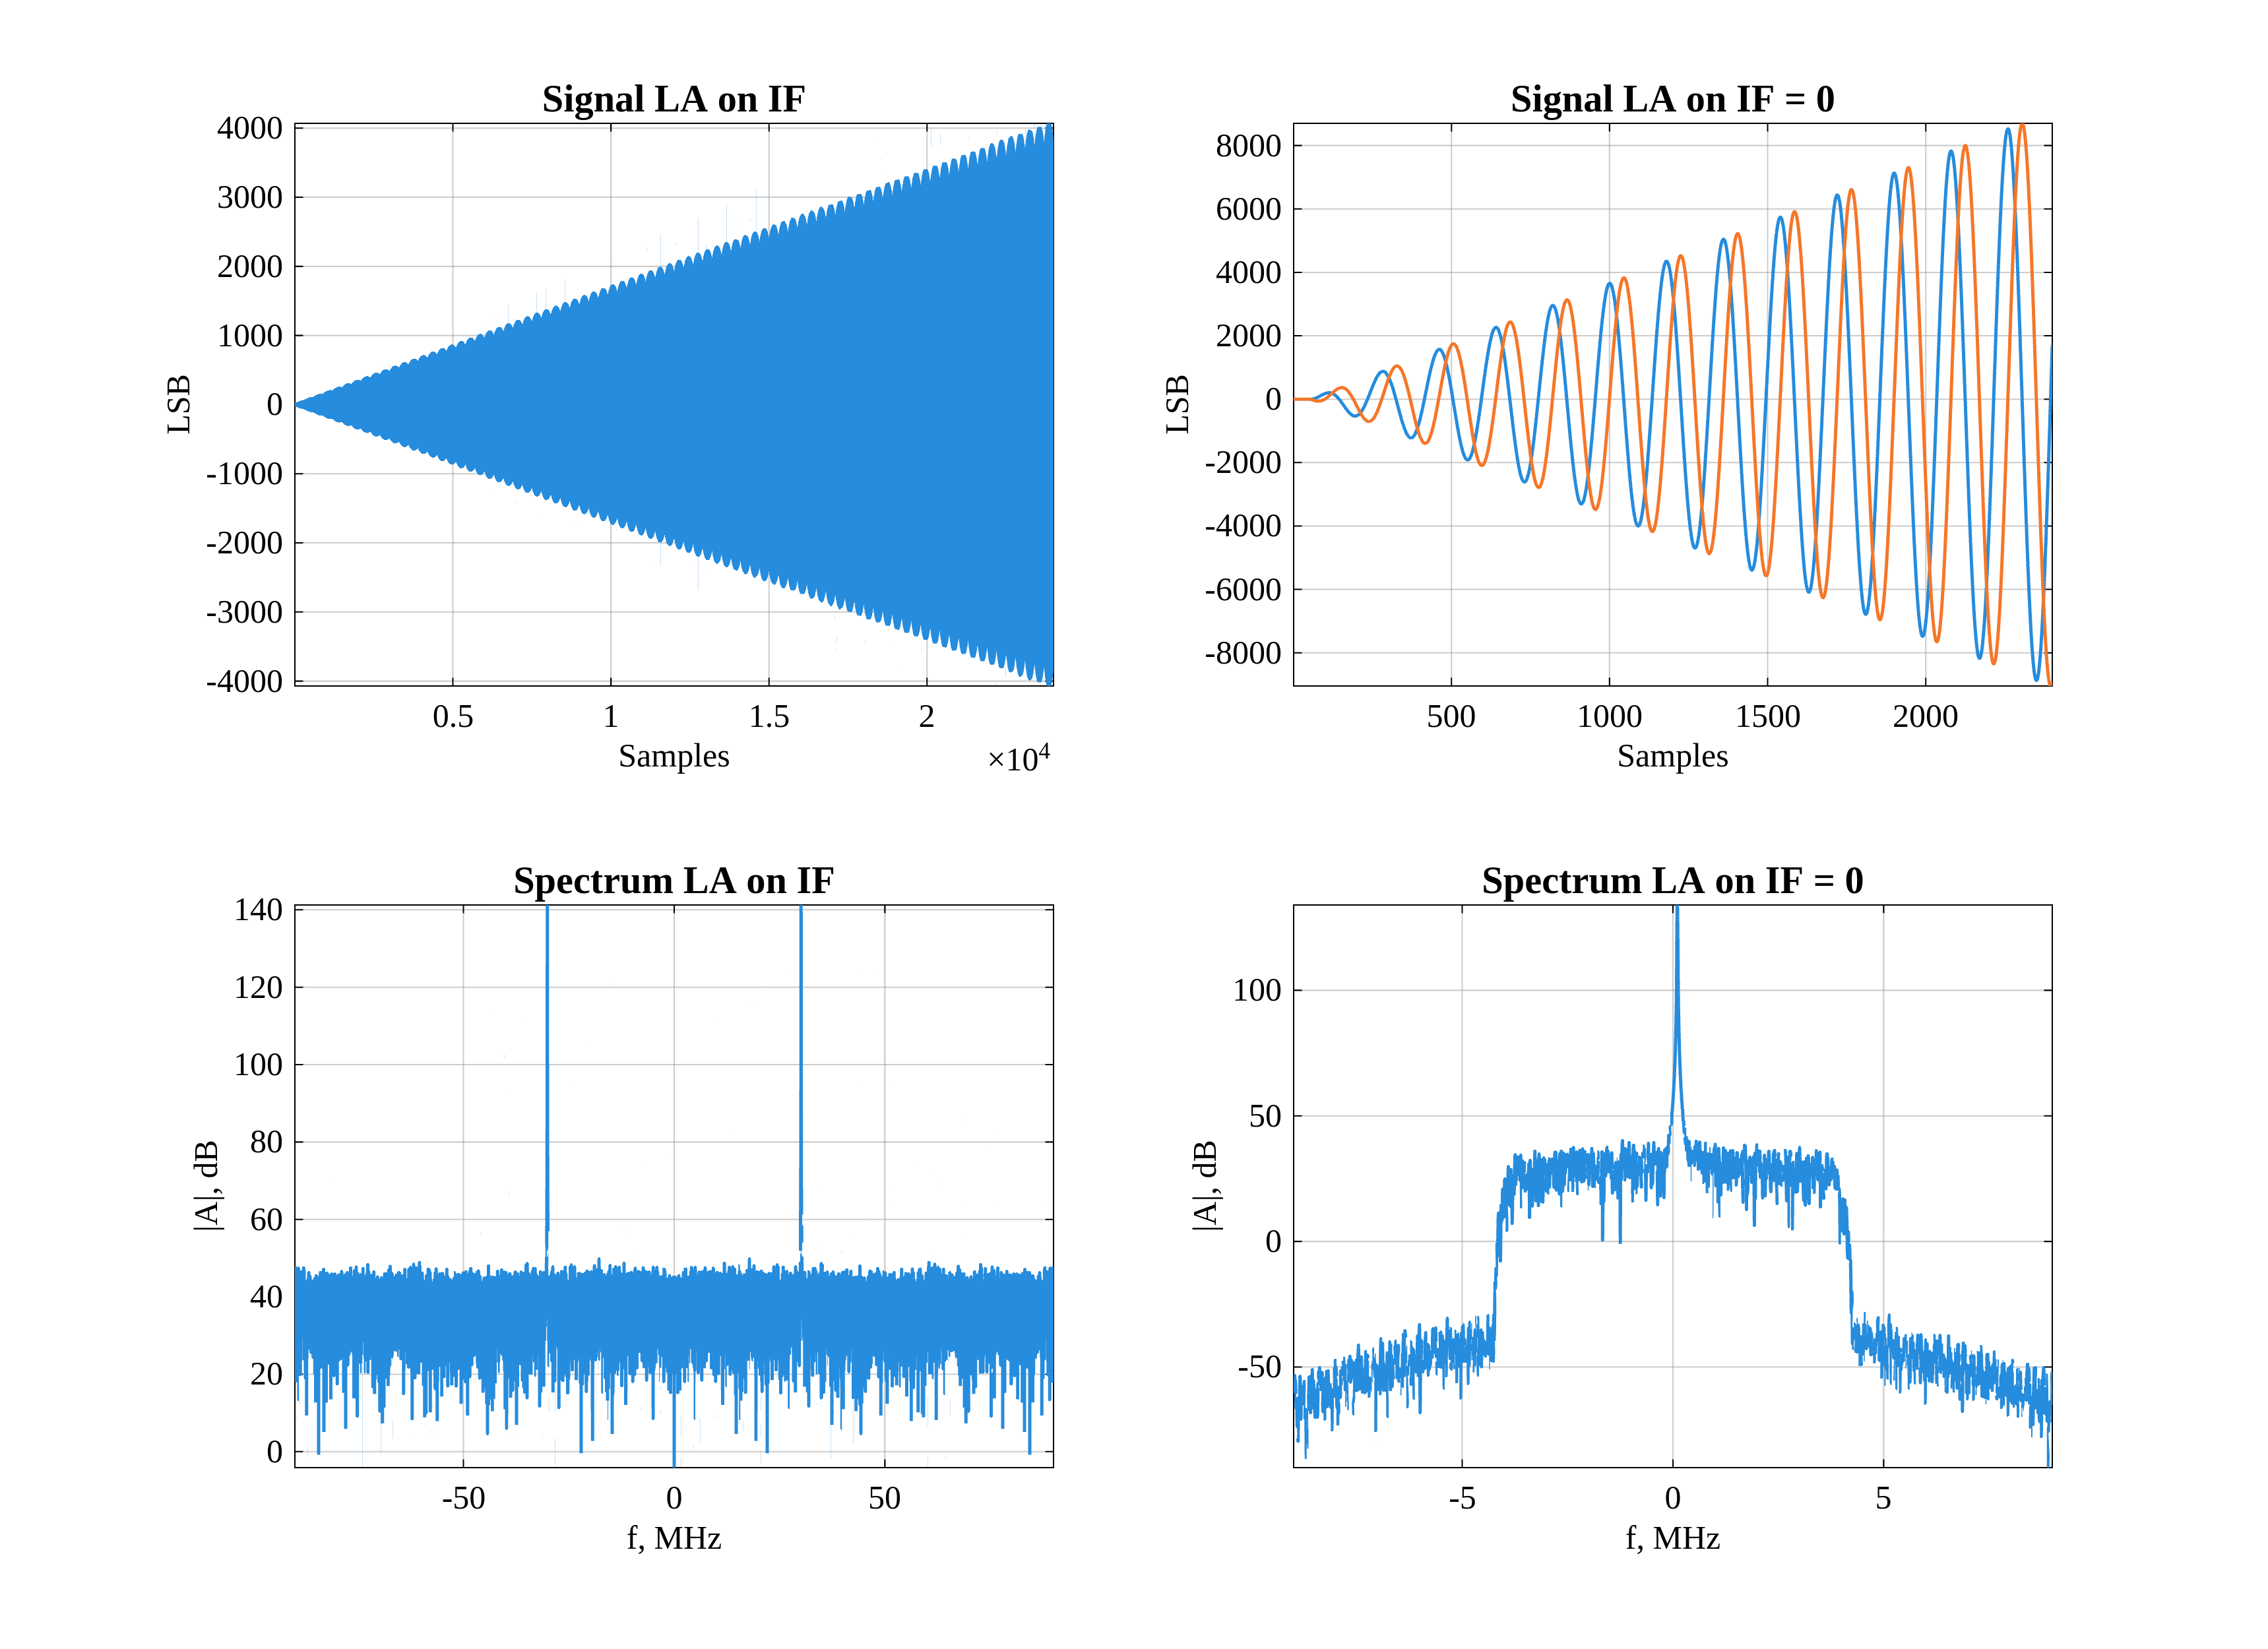
\includegraphics[width=0.85\textwidth]{export_figs/p5_linear_amplitude.png}
    \caption{Осциллограммы и спектры сигнала с линейно нарастающей амплитудой на промежуточной частоте и на видеочастоте}
    \label{fig:p5_lna}
\end{figure}

Форма огибающей выходного аналитического сигнала сохраняет строгую линейность во всем временном интервале без возникновения нелинейных искажений или переполнения разрядной сетки фильтров. Спектр выходного сигнала локализован в полосе пропускания каскада, подтверждая корректность масштабирования коэффициентов.

\subsection{Обработка широкополосного ЛЧМ-радиосигнала}

Исследование прохождения широкополосных сигналов проводилось с использованием радиоимпульса с линейной частотной модуляцией (ЛЧМ) с девиацией частоты в пределах рабочей полосы пропускания тракта. 

На рисунке \ref{fig:p6_in} показаны исходный комплексный видеосигнал ЛЧМ и сформированный входной радиосигнал. На рисунке \ref{fig:p6_out} представлены результаты демодуляции и фильтрации.

\begin{figure}[H]
    \centering
    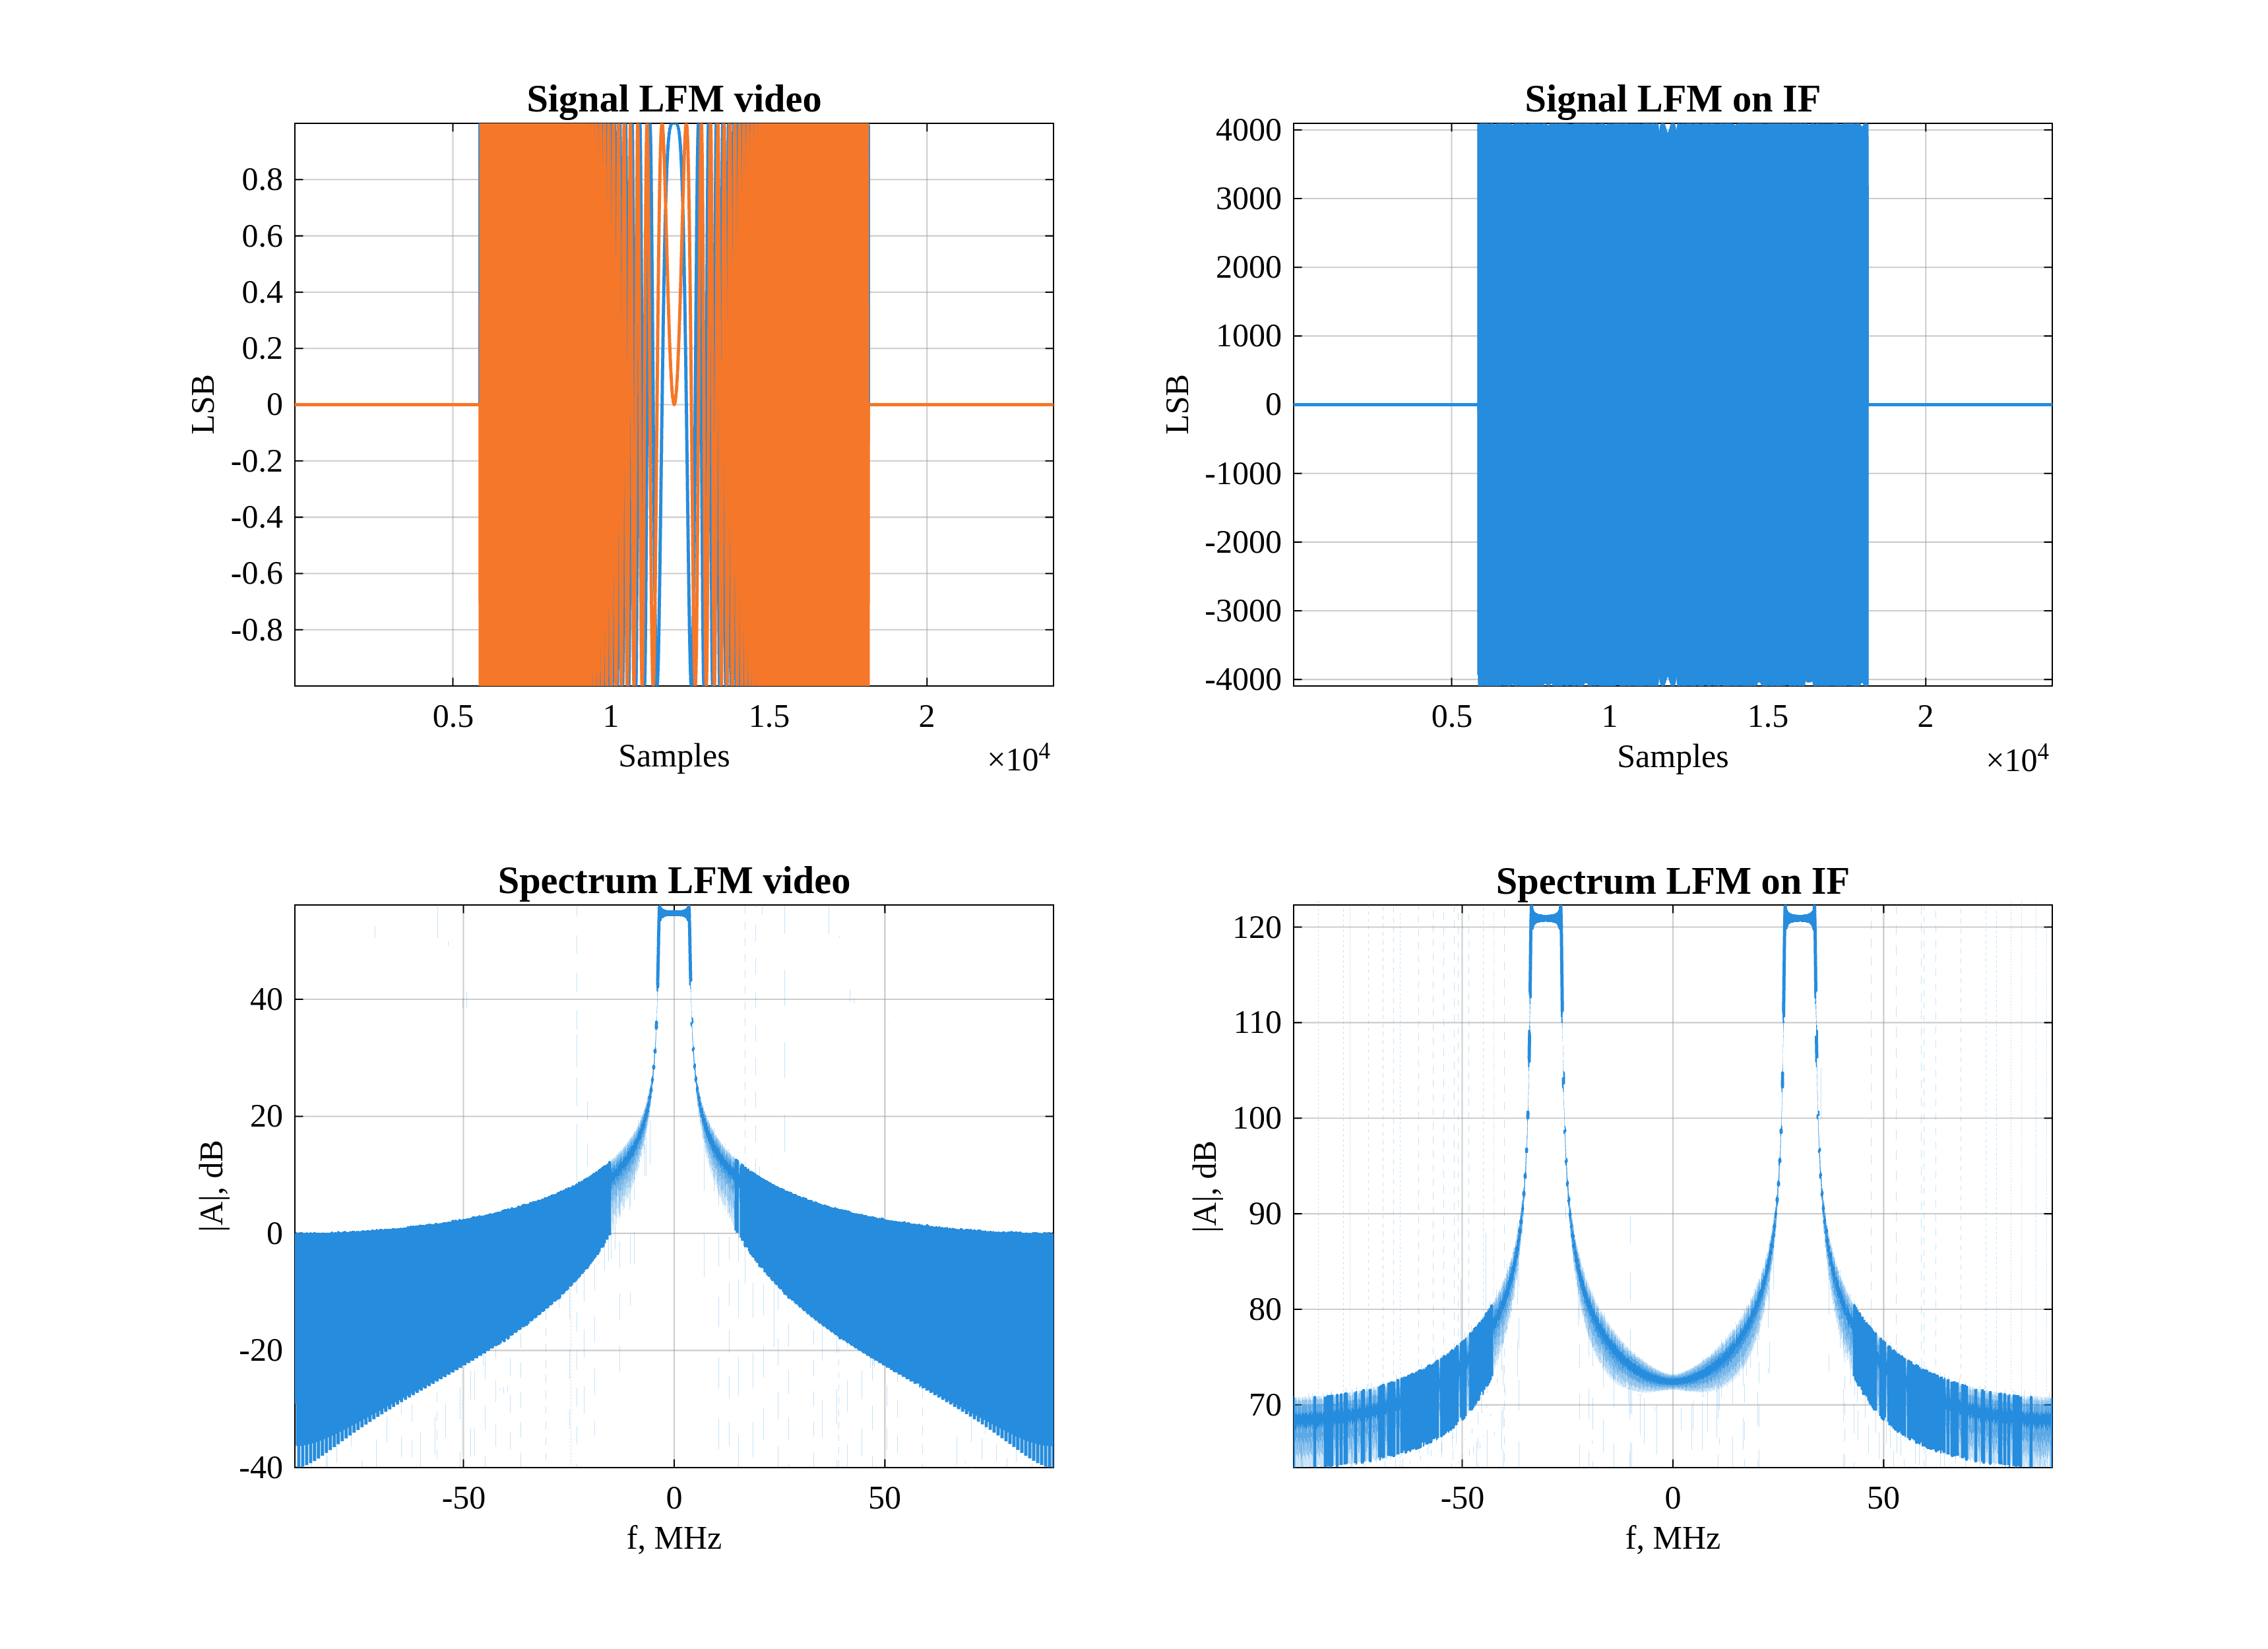
\includegraphics[width=0.85\textwidth]{export_figs/p6_lfm_input.png}
    \caption{Входной ЛЧМ-сигнал во временной и спектральной областях}
    \label{fig:p6_in}
\end{figure}

\begin{figure}[H]
    \centering
    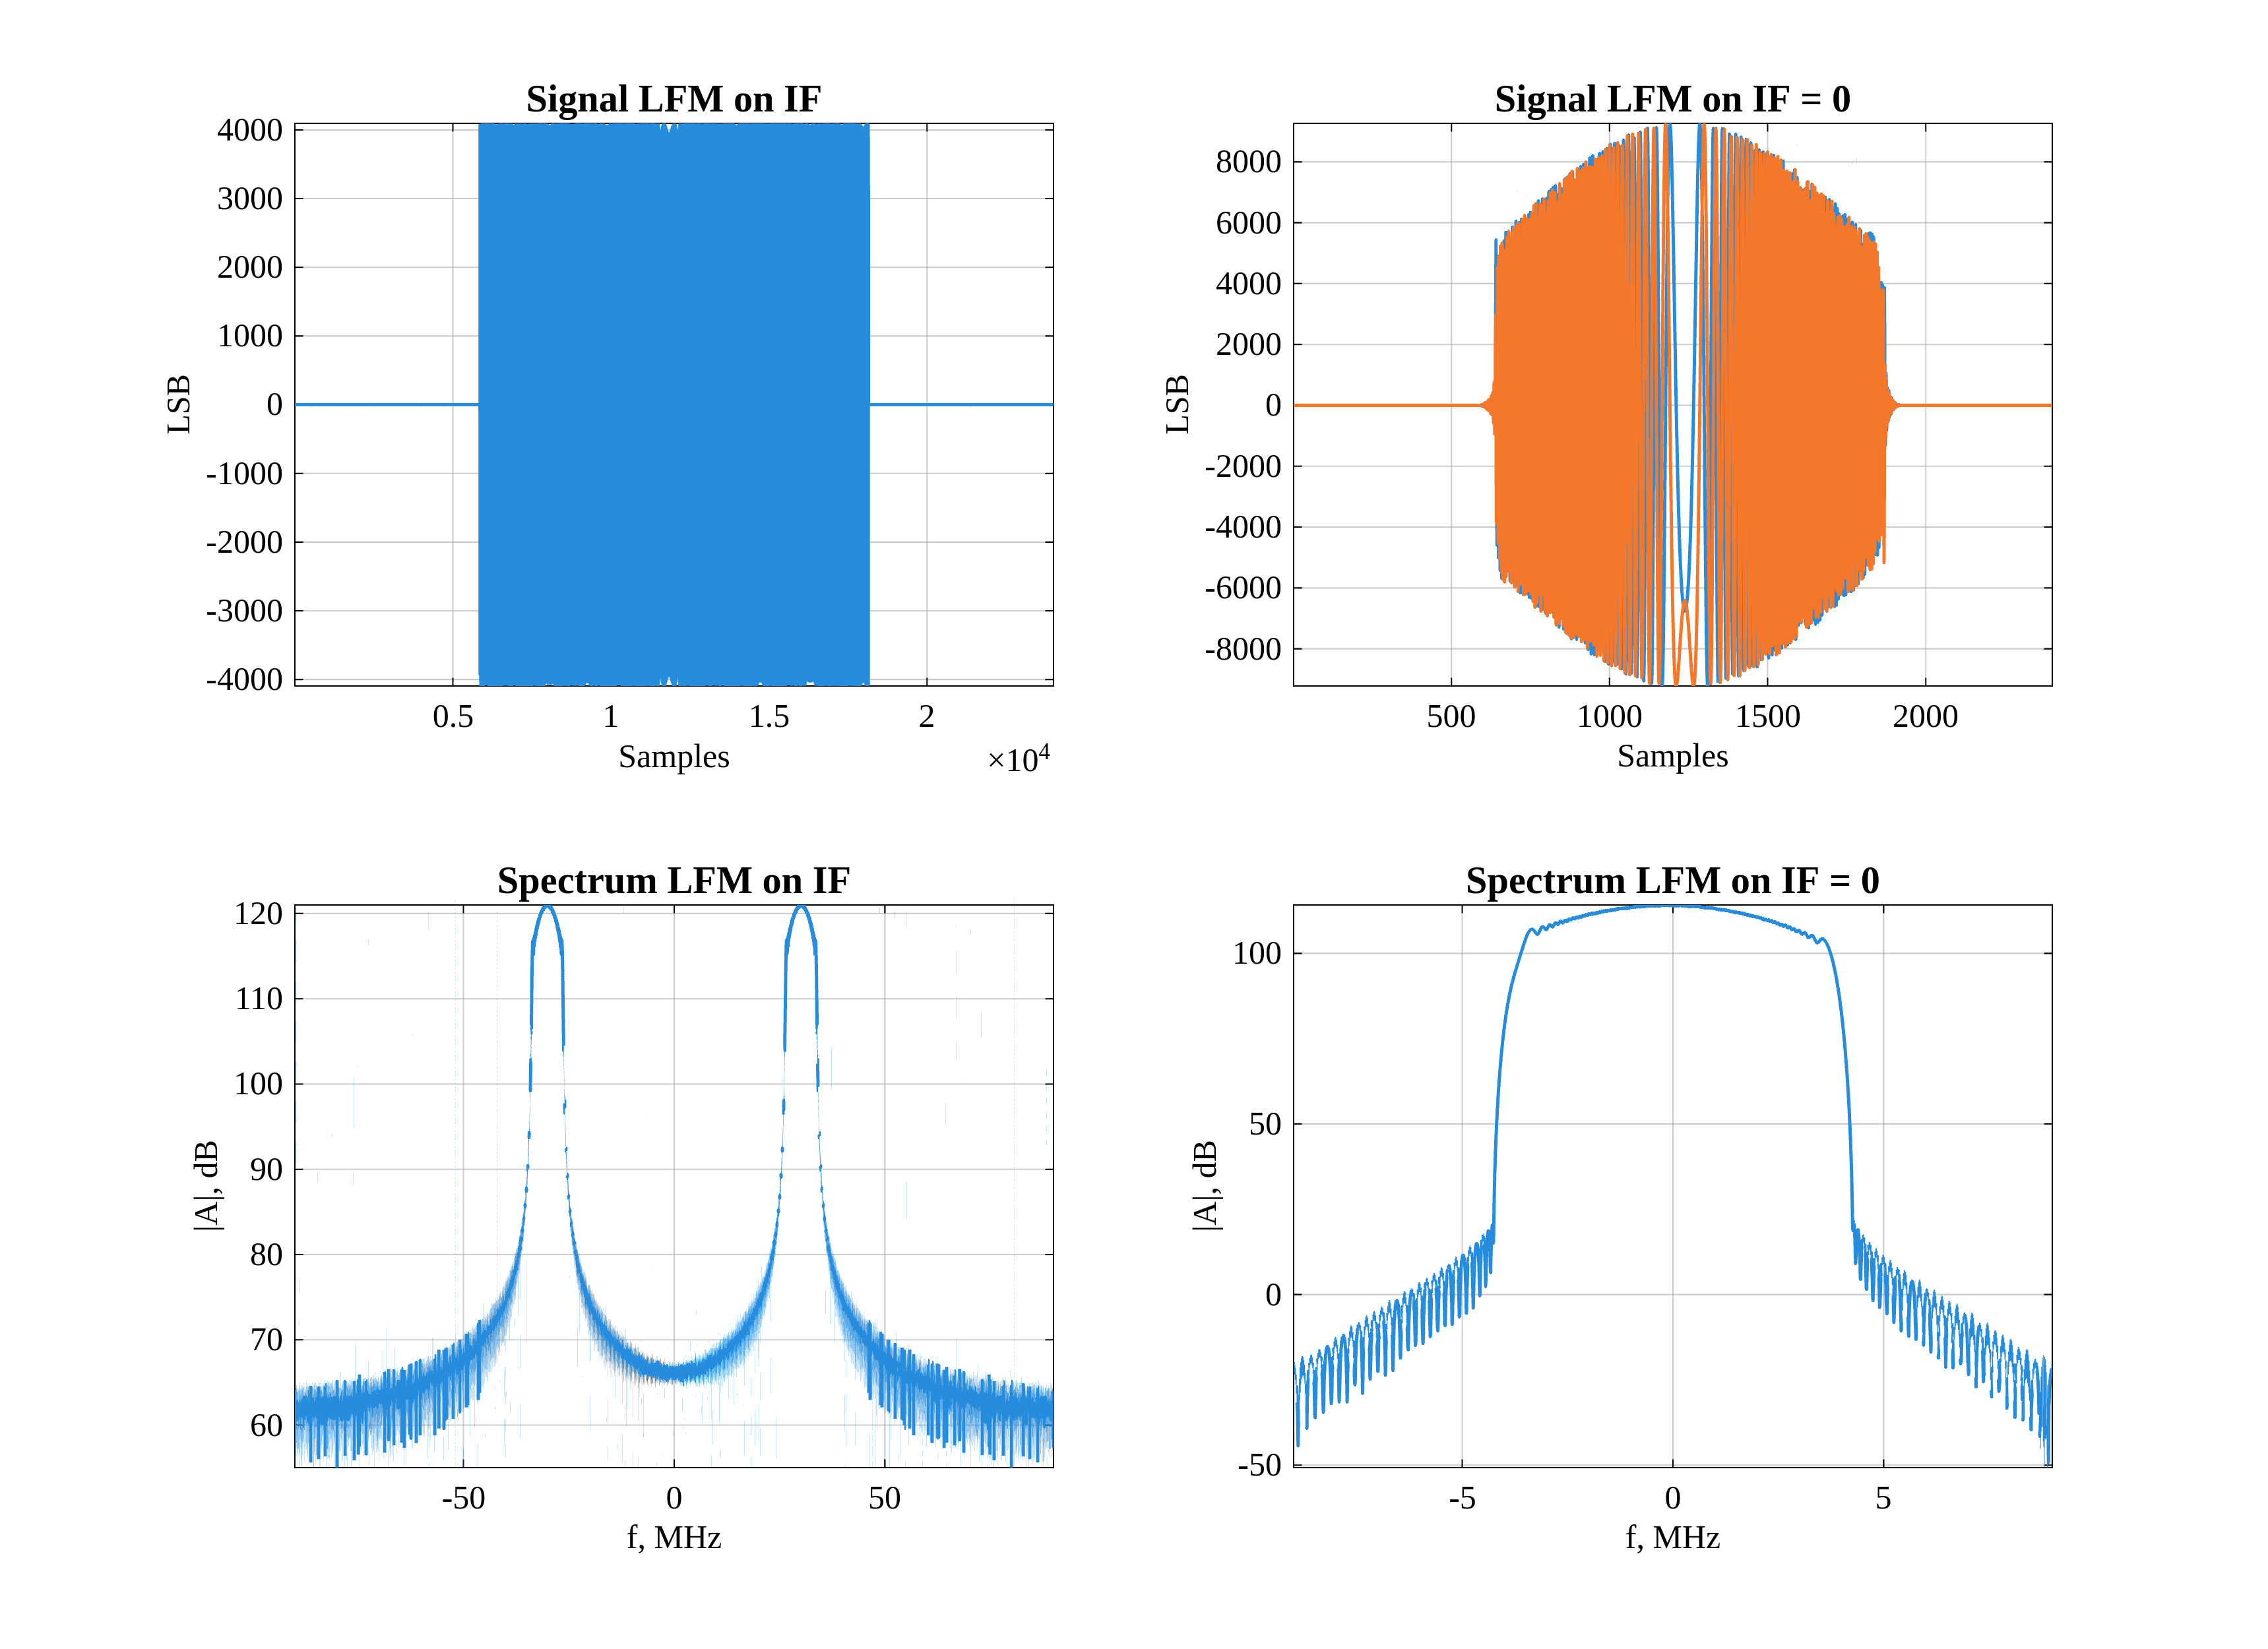
\includegraphics[width=0.85\textwidth]{export_figs/p6_lfm_output.png}
    \caption{Выходной ЛЧМ-сигнал после квадратурного переноса в ноль и децимации}
    \label{fig:p6_out}
\end{figure}

Выходной сигнал успешно перенесен на нулевую частоту. Спектральная плотность мощности ЛЧМ-радиосигнала полностью сохраняет прямоугольную форму в пределах рабочей полосы ($\approx 7.5$ МГц), а составляющие за ее пределами подавлены избирательным трактом более чем на 60 дБ.

\section{Сравнительный анализ каскадной и однократной фильтрации}

Для обоснования архитектуры тракта проведено сравнение каскадной схемы (децимирующий гребенчатый фильтр CIC совместно с корректирующим КИХ-фильтром) и эквивалентного одиночного КИХ-фильтра, выполняющего прореживание в $R=10$ раз за один шаг. Результаты сопоставления спектров приведены на рисунке \ref{fig:p7_comp}.

\begin{figure}[H]
    \centering
    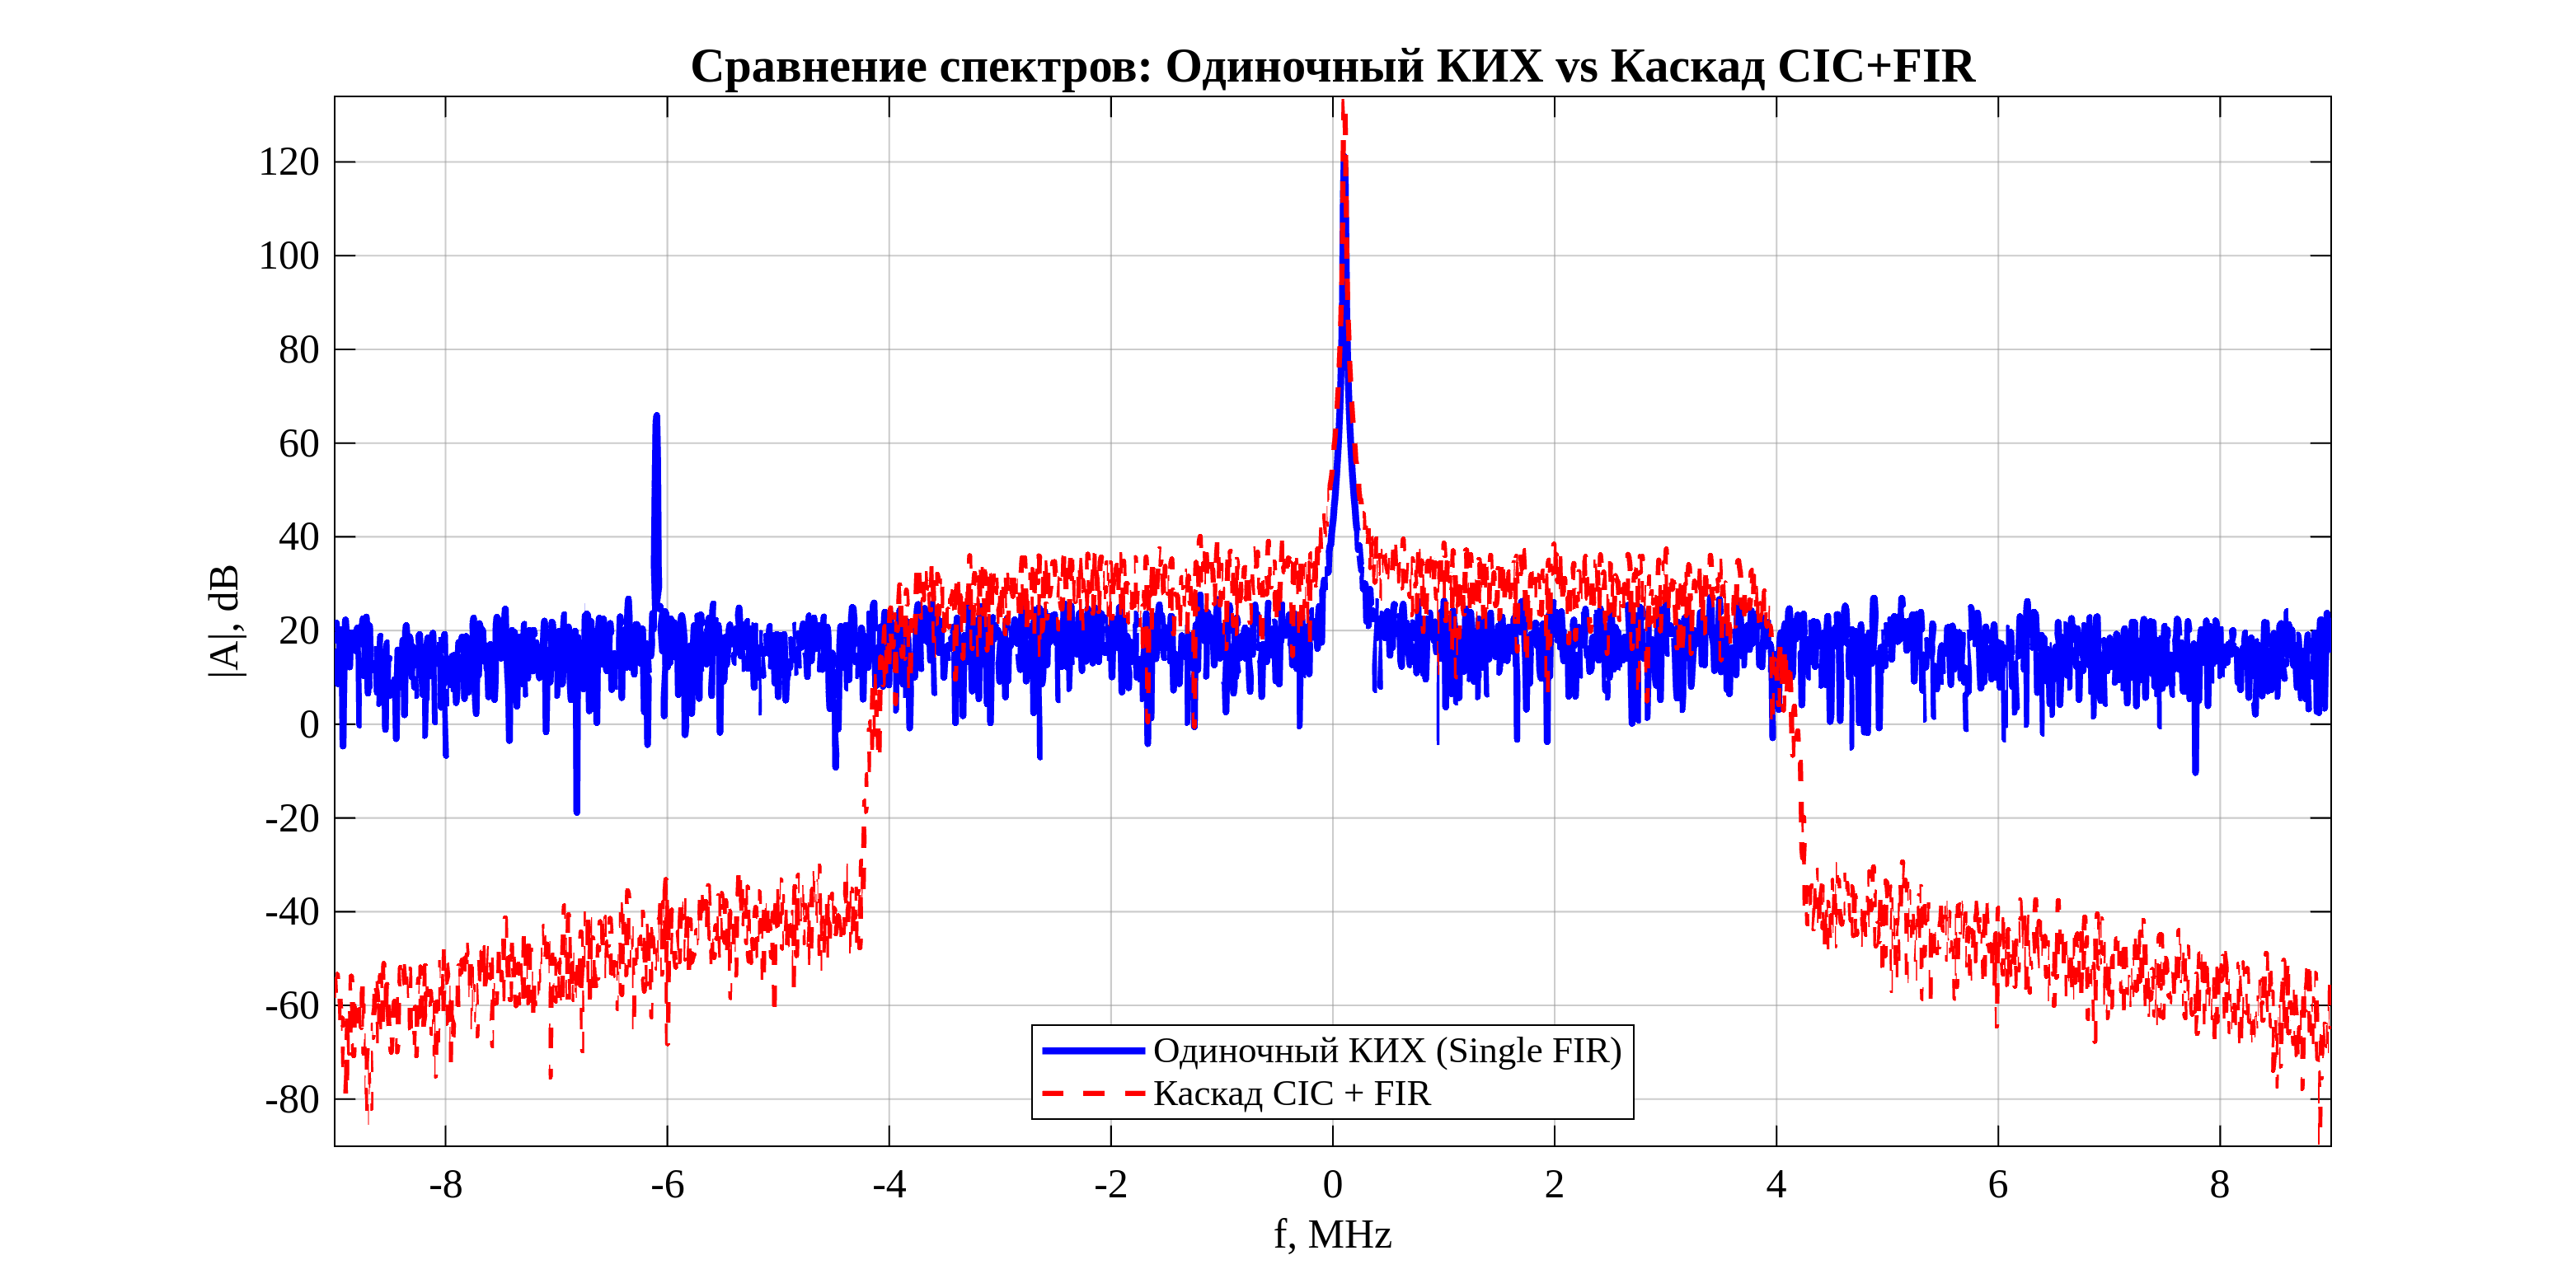
\includegraphics[width=0.9\textwidth]{export_figs/p7_single_fir_comparison.png}
    \caption{Сравнение спектров выходного сигнала для одиночного КИХ-фильтра и каскада CIC + КИХ}
    \label{fig:p7_comp}
\end{figure}

Сравнительный анализ спектральных характеристик показывает:
\begin{enumerate}
    \item В каскадной схеме децимации $\text{CIC} + \text{FIR}$ обеспечивается глубокое подавление шумов квантования вне рабочей полосы (уровень подавления превышает 60 дБ), а побочная составляющая суммарной частоты смесителя полностью устраняется.
    \item Одиночный КИХ-фильтр приемлемого порядка без предварительной фильтрации не обеспечивает требуемого ослабления в полосе заграждения (уровень внеполосного шума выше на 40--50 дБ). Кроме того, на частоте $-6.1$ МГц четко наблюдается неподавленный паразитный пик, обусловленный эффектом наложения спектров суммарной составляющей при децимации.
\end{enumerate}
